%! Author = leona
%! Date = 09/02/24
% !TeX root = ../thesis-main.tex

\chapter{Design}
\label{chap:design}
This chapter aims to give the reader a comprehensive view of this thesis' design. First, we will present the architectural design of the system, then we will shift the focus on
the detailed design, where the system will also be described in terms of behavior and interaction.

\section{Architectural Design}
\label{sec:architectural-design}
In this section, we will present and discuss RuFi's architectural design, shown in figure \ref{fig:rufi-architecture}.

\begin{figure}[ht!]
    \centering
    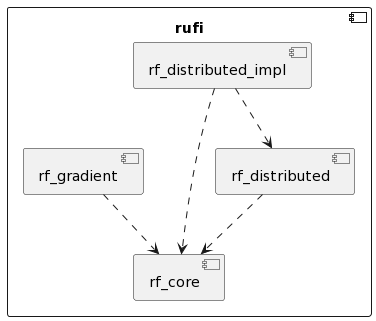
\includegraphics[width=0.6\textwidth]{figures/diagrams/img/rufi-architecture.png}
    \caption{RuFi's architectural design}
    \label{fig:rufi-architecture}
\end{figure}

In the figure, we can see the following components:

\begin{itemize}
    \item \textbf{rf-core}: this component defines key abstractions, such as the fundamental aggregate operators, builtins and a virtual machine;
    \item \textbf{rf-distributed}: this component defines concepts related to the distributed execution of aggregate programs.
          In particular, it defines core abstractions related to networking and message passing, as well as an implementation of the computational model discussed in \ref{par:comp-model};
    \item \textbf{rf-distributed-impl}: this component exposes a standard implementation for the concepts defined in \textbf{rf-distributed}.
          The choice of separating the abstraction definitions and the implementations in two modules will be discussed in chapter \ref{chap:implementation};
    \item \textbf{rf-gradient}: this component is a library exposing the gradient algorithm as an aggregate program.
\end{itemize}

\subsection{RuFi Core}
\label{subsec:rufi-core}
As mentioned in \ref{sec:architectural-design}, the module RuFi Core contains all the fundamental abstractions needed to start writing and evaluating aggregate programs.
Its structure is represented by the diagram in figure \ref{fig:rufi-core-architecture}.

\begin{figure}[ht!]
    \centering
    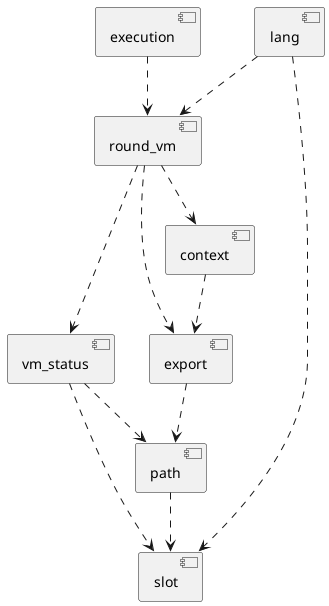
\includegraphics[width=0.5\textwidth]{figures/diagrams/img/rufi-core-architecture.png}
    \caption{RuFi Core's architectural design}
    \label{fig:rufi-core-architecture}
\end{figure}

\begin{itemize}
    \item \textbf{round\_vm}: This module defines a virtual machine for executing and evaluating aggregate programs and also other related concepts like the VM's status,
          the path, the execution context and the device exports, all of which will be discussed in more detail in section \ref{sec:detailed-design};
    \item \textbf{lang}: this module defines the fundamental aggregate operators, such as \textit{rep}, \textit{nbr}, \textit{foldhood}, \textit{branch} and some important builtin functions like \textit{foldhood plus} and \textit{mux};
    \item \textbf{macros}: this module exports some declarative macros that aim to simplify the writing of aggregate programs;\
    \item \textbf{execution}: this module contains functions for evaluating aggregate programs alongside the virtual machine.
\end{itemize}

\subsection{RuFi Distributed}
\label{subsec:rufi-distributed}
This module, as described in \ref{sec:architectural-design}, defines concepts related to the distributed execution of aggregate programs.
Its structure is represented by the diagram in figure \ref{fig:rufi-distributed-architecture}.

\begin{figure}[ht!]
    \centering
    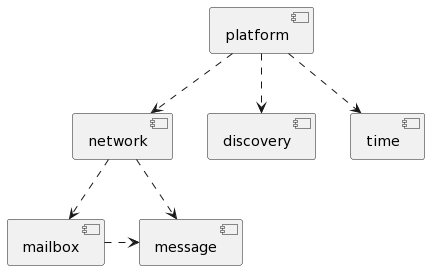
\includegraphics[width=0.7\textwidth]{figures/diagrams/img/rufi-distributed-architecture.png}
    \caption{RuFi Distributed's architectural design}
    \label{fig:rufi-distributed-architecture}
\end{figure}

In the diagram, we see the following elements:

\begin{itemize}
    \item \textbf{network}: this module defines abstractions for networking operations;
    \item \textbf{mailbox}: this module defines the logic of incoming message processing;
    \item \textbf{time}: this module defines some time-related operations that can be leveraged during the execution cycle;
    \item \textbf{discovery}: this module exposes traits for the discovery of possible neighbors and the logic for setting up neighboring sensors;
    \item \textbf{platform}: this module brings all the other functionalities together through the platform structure, which is responsible for managing the execution cycle of the aggregate programs;
\end{itemize}

\section{Detailed Design}
\label{sec:detailed-design}
This subsection aims to explain in more detail some design choices that are important to understanding the whole system.
After that, the system will be analyzed in terms of behavior and interaction.

\subsection{RuFi Core}
\subsubsection{Round VM}
The Round Virtual Machine is the operating heart of the RuFi framework. It is responsible for managing the state of the computation and generating the \ac{ast} of the aggregate program.
Each core language construct leverages the VM functionalities in its implementation.
In the class diagram in figure \ref{fig:round-vm-class}, we can see the elements that compose the VM.

\begin{figure}[ht!]
    \centering
    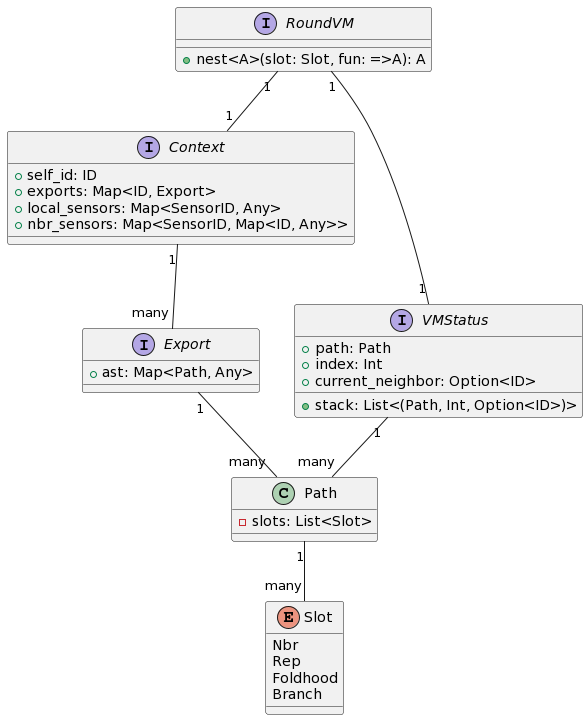
\includegraphics[width=0.7\textwidth]{figures/diagrams/img/round-vm-class.png}
    \caption{Round VM class diagram}
    \label{fig:round-vm-class}
\end{figure}

The Slot is a representation of a core construct of the \ac{ac} inside the \ac{ast}. A Path is a sequence of Slots, denoting a chain of aggregate operations.\\
A level above, the Export represents the entire \ac{ast} of the aggregate program, decorated with the value computed at each Path. The Export is also shared between neighbors during each
computation round.\\
The VMStatus encapsulates the execution state: it has a representation of the execution stack and the current Path being evaluated.\\
The Context represents the execution context for the device and contains relevant information such as the device identifier and the device's sensors alongside the exports of all the neighbors.
This means that during the computation process, each device has the \ac{ast} of its neighbors. This aspect is crucial to implement neighboring operations.\\
Above all, the RoundVM is responsible for generating the \ac{ast} and evaluate functions, and it does so with the \textit{nest} \ref{lst:nest} function, which gets executed whenever a core construct is called
and causes the VM to push a new Slot into the current Path. A more detailed explanation of this function will be given in chapter \ref{chap:implementation}.

\subsubsection{Language}
The language includes all the core constructs and built-in functions. Since each core construct call should grow the \ac{ast} by one Slot, each language construct and built-in function has
a dependency on the RoundVM, and so do the expressions that can be passed to them. This is reflected in their signatures, as shown in listing \ref{lst:lang}.

\lstinputlisting[language=Rust, label={lst:lang}]{listings/lang.rs}

\subsection{RuFi Distributed}
As mentioned before, the Distributed module of RuFi has the goal of enabling the distributed execution of aggregate programs. A key concept defined in this module to reach this goal is the Platform.
This structure is responsible for managing the execution cycle of aggregate programs, as well as the communication between neighbors, and it does so by leveraging the other concepts defined in the module.
A representation of the main concepts in the module is shown in figure \ref{fig:distributed-class}.

\begin{figure}[ht!]
    \centering
    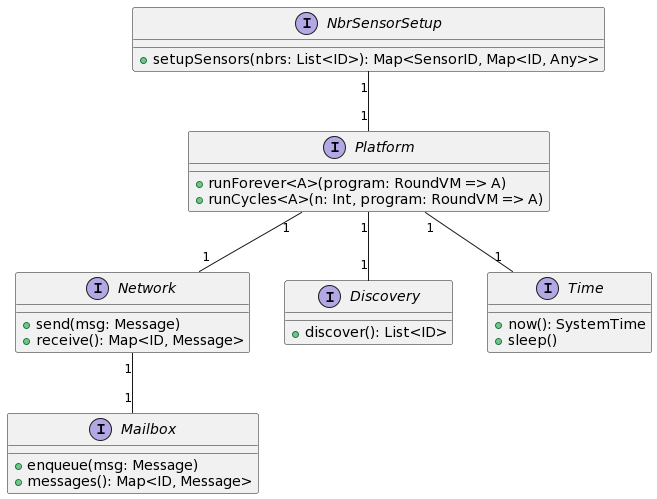
\includegraphics[width=0.7\textwidth]{figures/diagrams/img/rufi-distributed-class.png}
    \caption{RuFi Distributed class diagram}
    \label{fig:distributed-class}
\end{figure}

A more detailed explanation of the module's components' functioning will be given in sections \ref{subsec:behavior} and \ref{subsec:interaction}.

\subsection{Behavior}
\label{subsec:behavior}
In this section, we will showcase the behavior of a device when executing an aggregate program, which is represented by the activity diagram in figure \ref{fig:behavior}.

\begin{figure}[ht!]
    \centering
    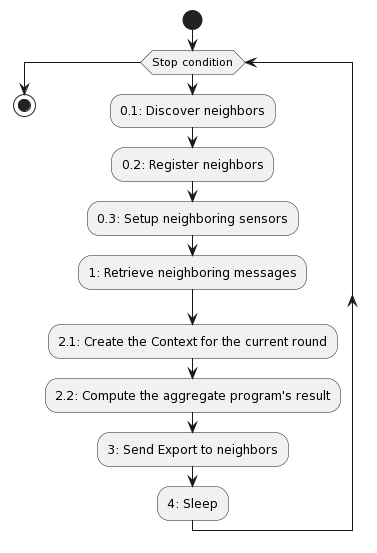
\includegraphics[width=0.5\textwidth]{figures/diagrams/img/platform-activity.png}
    \caption{Device behavior}
    \label{fig:behavior}
\end{figure}

The activities represented in the diagram \ref{fig:behavior} closely resemble the computational model in \ref{par:comp-model}.
It is worth noting that the proposed behavior represents a synchronous execution cycle, where all the steps are performed in a sequential order. It is possible to extend this design
to support the asynchronous execution of some of the steps like the discovery process, which could be done in parallel with the computation cycle. However, this solution would require the employment of an asynchronous runtime, which is a requirement that can be costly for certain device architectures. As such, the proposed design
takes into account the synchronous case, leaving the asynchronous one to future developments.

\subsection{Interaction}
\label{subsec:interaction}

In this section, we will describe the interaction between devices during the distributed execution of an aggregate program, focusing in particular on the networking operations design.
Although there is no strict requirement for the communication protocol between devices, the proposed design models the interaction between nodes via a publish-subscribe model akin to the one used in popular protocols like MQTT.
As such, the following sequence diagrams will feature a Broker participant, whose design falls out of this thesis' scope, who is responsible for forwarding and broadcasting messages between devices.

\subsubsection{Network Creation}
The behavior of the system when a device is added to the network is represented by the sequence diagram in figure \ref{fig:network-creation}.

\begin{figure}[ht!]
    \centering
    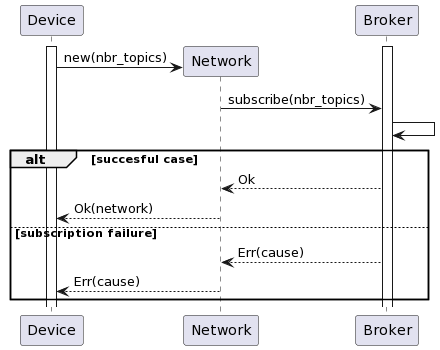
\includegraphics[width=0.7\textwidth]{figures/diagrams/img/activity-network-creation.png}
    \caption{Network creation}
    \label{fig:network-creation}
\end{figure}

\begin{enumerate}
    \item The device first instantiates a new Network with an initial list of discovered neighbor topics;
    \item The Network subscribes to the neighbors' topics via the Broker;
    \item If the subscription is successful, a reference to the Network is returned to the device; if not, an \texttt{Err} is returned instead.
\end{enumerate}

\subsubsection{Message Passing}
The behavior of the system when a device sends a message to its neighbors is represented by the sequence diagram in figure \ref{fig:message-passing}.

\begin{figure}[ht!]
    \centering
    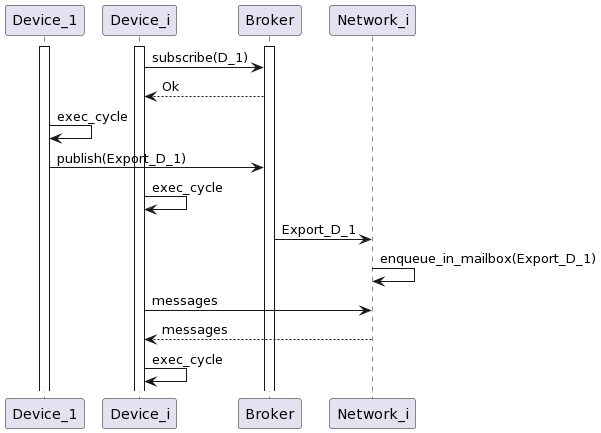
\includegraphics[width=0.7\textwidth]{figures/diagrams/img/activity-message-passing.png}
    \caption{Message passing}
    \label{fig:message-passing}
\end{figure}

\begin{enumerate}
    \item The Device i subscribes to the topic of Device 1;
    \item when Device 1 publishes a message, the Broker forwards it to Device i via its Network instance;
    \item when Device i starts a new computation cycle, one of the first steps is to check the mailbox for incoming messages;
    \item the Device i finds among other messages the one sent from Device 1, adding the Export it to its Context for the current computation cycle.
\end{enumerate}
